\documentclass{beamer}
%
% Choose how your presentation looks.
%
% For more themes, color themes and font themes, see:
% http://deic.uab.es/~iblanes/beamer_gallery/index_by_theme.html
%
\mode<presentation>
{
  \usetheme{Warsaw}      % or try Darmstadt, Madrid, Warsaw, ...
  \usecolortheme{beaver} % or try albatross, beaver, crane, ...
  \usefonttheme{serif}  % or try serif, structurebold, ...
  \setbeamertemplate{navigation symbols}{}
  \setbeamertemplate{caption}[numbered]
} 

\setbeamertemplate{background}
%{\includegraphics[width=\paperwidth,height=\paperheight,keepaspectratio]{5.jpg}}


\usepackage{amsmath,amssymb}
\usepackage[english]{babel}
\usepackage[utf8x]{inputenc}
\usepackage{xcolor}% http://ctan.org/pkg/xcolo
%\usepackage{xcolor}
\usepackage{listings}
\usepackage[english]{babel}

\usepackage{tikz}
\usepackage{subcaption}
\usepackage{tkz-tab}
\usepackage{caption}
\usepackage{latexsym}
%\usepackage[british]{babel}
\usepackage{hhline}
\usepackage{multirow}
\usepackage[figurename=Fig]{caption}
\usetikzlibrary{matrix,positioning,decorations.pathreplacing,calc}
\usepackage{adjustbox}

\usetikzlibrary{arrows,shapes}

% Set various styles for the matrices and braces. It might pay off to fiddle around     with the values a little bit
 \pgfkeys{tikz/mymatrixenv/.style={decoration=brace,every left delimiter/.style=    {xshift=3pt},every right delimiter/.style={xshift=-3pt}}}
 \pgfkeys{tikz/mymatrix/.style={matrix of math nodes,left delimiter=[,right delimiter=    {]},inner sep=1pt,column sep=0.5em,row sep=0.5em,nodes={inner sep=0pt}}}
 \pgfkeys{tikz/mymatrixbrace/.style={decorate,thick}}
 \newcommand\mymatrixbraceoffseth{0.5em}
 \newcommand\mymatrixbraceoffsetv{0.2em}

% Now the commands to produce the braces. (I'll explain below how to use them.)
\newcommand*\mymatrixbraceright[4][m]{
\draw[mymatrixbrace] ($(#1.north west)!(#1-#3-1.south west)!(#1.south west)-    (\mymatrixbraceoffseth,0)$)
    -- node[left=2pt] {#4} 
    ($(#1.north west)!(#1-#2-1.north west)!(#1.south west)-(\mymatrixbraceoffseth,0)$);
}
 \newcommand*\mymatrixbraceleft[4][m]{
 \draw[mymatrixbrace] ($(#1.north east)!(#1-#2-1.north east)!(#1.south east)+    (\mymatrixbraceoffseth,0)$)
    -- node[right=2pt] {#4} 
     ($(#1.north east)!(#1-#3-1.south east)!(#1.south east)+    (\mymatrixbraceoffseth,0)$);
}
\newcommand*\mymatrixbracetop[4][m]{
\draw[mymatrixbrace] ($(#1.north west)!(#1-1-#2.north west)!(#1.north east)+(0,\mymatrixbraceoffsetv)$)
    -- node[above=2pt] {#4} 
    ($(#1.north west)!(#1-1-#3.north east)!(#1.north east)+(0,\mymatrixbraceoffsetv)$);
}
\newcommand*\mymatrixbracebottom[4][m]{
\draw[mymatrixbrace] ($(#1.south west)!(#1-1-#3.south east)!(#1.south east)-(0,\mymatrixbraceoffsetv)$)
    -- node[below=2pt] {#4} 
    ($(#1.south west)!(#1-1-#2.south west)!(#1.south east)-(0,\mymatrixbraceoffsetv)$);
}

\usepackage{amsthm}
 
\definecolor{OliveGreen}{rgb}{0.2,0.7,0.2}
\definecolor{airforceblue}{rgb}{0.36, 0.54, 0.66}
\definecolor{awesome}{rgb}{1.0, 0.13, 0.32}
\definecolor{brilliantrose}{rgb}{1.0, 0.33, 0.64}
\definecolor{charcoal}{rgb}{0.21, 0.27, 0.31}
	\definecolor{britishracinggreen}{rgb}{0.0, 0.26, 0.15}
    \definecolor{darkgreen}{rgb}{0.0, 0.2, 0.13}
    \definecolor{darkpastelgreen}{rgb}{0.01, 0.75, 0.24}
    \definecolor{lavenderindigo}{rgb}{0.58, 0.34, 0.92}
\theoremstyle{definition}
%\newtheorem{definition}{Definition}[section]
 
\tikzset{
    small-node/.style={
        shape=rectangle,
        fill=white,
        draw,
        minimum size=+4mm}
}

\theoremstyle{remark}
\newtheorem*{remark}{Remark}
 
 \newcommand{\booleans}{\mathbb{B}}
\newcommand{\naturals}{\mathbb{N}}
\newcommand{\integers}{\mathbb{Z}}
\newcommand{\ordinals}{\mathbb{O}}
\newcommand{\numarals}{\mathbb{I}}

\lstset
{
    language=[LaTeX]TeX,
    breaklines=true,
    basicstyle=\tt\scriptsize,
    %commentstyle=\color{green}
    keywordstyle=\color{blue},
    %stringstyle=\color{black}
    identifierstyle=\color{red},
}

\title[SASB 2017]{SMT Solving for Vesicle Traffic Systems in Cells}
%\author{A. Gupta, A. Shukla, M. Srivas, and M. Thattai}
%\institute{ISR/IST}
\author[A.Gupta, A.Shukla, M.Srivas, M.Thattai]{A. Gupta\inst{1}\and\textbf{A. Shukla}\inst{2} M. Srivas\inst{2}\and M. Thattai \inst{3}}
\institute[shortinst]{\inst{1} TIFR, Mumbai \and %
                      \inst{2} CMI, Chennai \and %
                      \inst{3} NCBS, Bangalore %
                      }
\date{August 29, 2017}

\AtBeginSection[]
{
  \begin{frame}<beamer>
    \frametitle{Outline}
    \tableofcontents[currentsection,currentsubsection]
  \end{frame}
}

\begin{document}

\begin{frame}
  \titlepage
\end{frame}


\addtobeamertemplate{navigation symbols}{}{%
    \usebeamerfont{footline}%
    \usebeamercolor[fg]{footline}%
    \hspace{1em}%
    \insertframenumber
}
\setbeamertemplate{headline}[page number]


% Uncomment these lines for an automatically generated outline.
\begin{frame}{Outline}
  \tableofcontents
\end{frame}


\section{Interesting question and background}
%  \usebackgroundtemplate{%             declare it
% \tikz[overlay,remember picture] \node[opacity=0.8, at=(current page.south)] {
%     \includegraphics[height=4.0cm]{5.png}};
%  }
\begin{frame}{An interesting question}
%\usebackgroundtemplate{ }    %% undeclare it

{\color{blue}{Biological interest:}}
	What is the form of an eukaryotic membrane traffic?\newline
% \begin{figure}
%    				\includegraphics[height=4.0cm]{222.png}
%  \end{figure}
% \center Figure from Mani's recent paper \cite{mani2016stacking}.
\end{frame}


%\section{Some biology}

\begin{frame}{Vesicular Transport in eukaryotic }
	\begin{columns}
		\begin{column}{4cm}
			\begin{figure}
             \begin{tikzpicture}
                 \node<1> (img1) {\begin{tikzpicture}
                        \foreach \i in {0,...,2}
                            \foreach \j in {0,...,2}
	                            \node [small-node] (n-\i\j) at (\i + 0.50*rand + 1,\j + 0.50*rand + 1) {$n_{\value{\i} + \value{\j}}$};
            \end{tikzpicture}};
                 \node<2> (img2) {
                 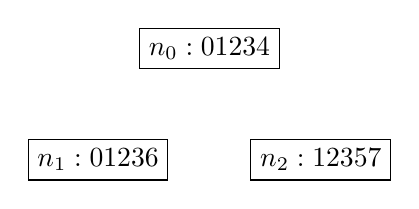
\begin{tikzpicture}[node distance = 20mm]
%   \node[draw] (n0) {$n_0:012$};
%   \node[draw,right of=n0] (n1) {$n_1:123$};
  \node[draw] (n0) {$n_0:01234$};
  \node[draw,below left of=n0] (n1) {$n_1:01236$};
  \node[draw,below right of=n0] (n2) {$n_2:12357$};
  
\end{tikzpicture}             };
                 \node<3> (img3) {
                 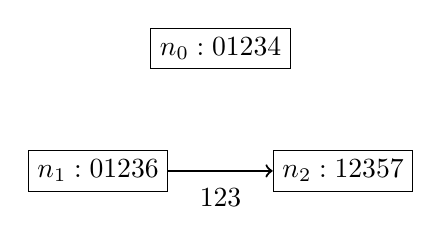
\begin{tikzpicture}[node distance = 22mm]
%                     \node[draw] (n0) {};
%                     \node[draw,right of=n0] (n1) {};
%   \draw[->,thick] (n0) -- node[above=1mm]  {$12$} (n1);
 \node[draw] (n0) {$n_0:01234$};
  \node[draw,below left of=n0] (n1) {$n_1:01236$};
  \node[draw,below right of=n0] (n2) {$n_2:12357$};
  \draw [->,thick] (n1) -- node[below=1mm]  {$123$} (n2);

\end{tikzpicture}                 
                 };
           \end{tikzpicture}

	      \end{figure}
		\end{column}
		\begin{column}{6cm}
			\begin{itemize}
				\item Cells consist of compartments (nodes) ∼10
				\pause
				\item Compartments contain molecules (labels)
				\pause
				\item Molecules moves around via “transfer vesicles” among compartments. (edges label represent transferred molecules)
%(edges labelled with the transferred molecules)
			\end{itemize}
		\end{column}
    \end{columns}
    
\end{frame}

\begin{frame}

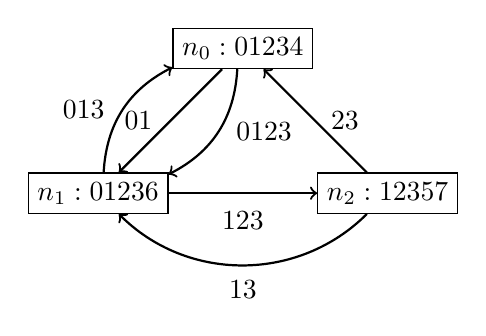
\begin{tikzpicture}[node distance = 26mm]
  \node[draw] (n0) {$n_0:01234$};
  \node[draw,below left of=n0] (n1) {$n_1:01236$};
  \node[draw,below right of=n0] (n2) {$n_2:12357$};
  
  \draw[->,thick] (n0) -- node[left=1mm]  {$01$} (n1);
  \draw [->,thick] (n0) to [bend right=-30] node[right=1mm]  {$0123$} (n1);
  \draw [->,thick] (n1) to [bend right=-30] node[left=1mm]  {$013$} (n0);

  \draw [->,thick] (n1) -- node[below=1mm]  {$123$} (n2);
  \draw [->,thick] (n2) to [bend right=-45] node[below=2pt]  {$13$} (n1);

  \draw [->,thick] (n2) -- node[right=2pt]  {$23$} (n0);
\end{tikzpicture}

\vspace{1cm}

{\color{red} {VTS ≡ labeled directed graph}}
that follows certain biological rules.
% \begin{tikzpicture}[node distance = 26mm]
%   \node[draw] (n0) {$n_0:012$};
%   \node[draw,right of=n0] (n1) {$n_1:123$};
%   \draw[->,thick] (n0) -- node[left=1mm]  {$12$} (n1);
% \end{tikzpicture}    

\end{frame}


\section{Constraint solving}
	
\begin{frame}{Problem?}
\begin{itemize}

\item Find a VTS that satisfies some biological rules.\newline 
\usebackgroundtemplate{ }    %% undeclare it

\pause
\item Solution?
\pause 
Easy... \newline
\pause
\item Encode rules as combinatorial constraints and {\color{blue}{use SAT/SMT solvers}} \newline
\pause 
\item However, VTS is most complex network in cells [mani 16], so encoding is \textbf{treacherous!}
\end{itemize}
\pause
\vskip 1cm
Contribution:
{\color{red}{an effective encoding.}}
\end{frame}

\section{Constraints}

\begin{frame}
\frametitle{Find VTS that satisfied these constraints}
\begin{enumerate}
\item {\color{blue} {``Activity constraint"}}.. \\

\item \textbf{Fusion constraint} \\

\item Pairing function. \\ 

\item Steady state constraint. \\

\item Connectivity constraint. \\

\end{enumerate}
\end{frame}

\begin{frame}
\begin{itemize}
        	\item {\color{blue} {``Activity constraint"}}: a molecule may or may not be {\color{brilliantrose}{active}} on the edge/nodes. 
\end{itemize} 
\end{frame}
            
     \begin{frame}
\begin{itemize}
            \item {\color{blue} {``Fusion constraint"}}: each edge must have \textbf{an active molecule that “fuses” with some active molecule at its destination node}.
                 \end{itemize} 
\end{frame}

 \begin{frame}
\begin{itemize}
            \item {\color{blue} {``Pairing function"}}: the fusing pair must be {\color{brilliantrose}{unique}} for each edge; 
                     \end{itemize} 
\end{frame}
\begin{frame}
\begin{itemize}
            \item {\color{blue} {``Steady state constraint"}}: all molecules must \textbf{move around in closed cycles}.
            \end{itemize} 
\end{frame}

\begin{frame}
\begin{itemize}

     \item {\color{blue} {``Connectivity constraint"}}: resulting graph is not \textbf{k-connected}. 
           
		\end{itemize}
\end{frame}


%	\begin{frame}{Find VTS that satisfied these constraints}
    
% 		\begin{itemize}
%         	\item A molecule may or may not be {\color{brilliantrose}{active}} on the edge/nodes; {\color{blue} {``activity constraint"}}.
%        %     \pause
%             \item Each edge must have \textbf{an active molecule that “fuses” with some active molecule at its destination node}; {\color{blue} {``fusion constraint"}}.
%       %                  \pause
%             \item The fusing pair must be {\color{brilliantrose}{unique}} for each edge; {\color{blue} {``pairing function/matrix"}}
%        %                 \pause

%             \item All molecules must \textbf{move around in closed cycles}; {\color{blue} {``steady state constraint"}}.
%            \pause
%             \item Resulting graph is not \textbf{k-connected}. {\color{blue} {``connectivity constraint"}}
           
% 		\end{itemize}
% 	\end{frame}

	\begin{frame}{Formal VTS}
    \theoremstyle{Formal VTS}
    	A \emph{Formal VTS} is a tuple
\begin{definition}{}
G = (N, M, E, L, P, f).
\end{definition}

%\[ A=(N, M, E, L, P, F )\ ,\]
where
\begin{itemize}

\item $N$ set of \emph{nodes} representing compartments.

\item $M$ is a different type of \emph{molecules} in the system.

\item $E$ is the set of edges with molecule sets as \textit{labels}.
%E $\subseteq$ N $\times$ ($2^{M}$ − $\phi$) $\times$ N  %\pause 
%\hspace{0.5cm} $\pmb{2^{2N + M}}$

\item $L$ is the set of \emph{node labels}.
%N $\to$ $2^{M}$ 
%\pause  \hspace{0.5cm} $\pmb{2^{M}}$
\pause

\item {\color{darkgreen}{$P$ is the \emph{pairing relation}}}.
%P $\subseteq$ M $\times$ M 
%\pause \hspace{0.5cm} $\pmb{2^{2M}}$

\item $f: M\to \wp(M) \to \booleans$ are the \emph{activity maps}. 
%\pause \hspace{0.5cm} $\pmb{2^{2 ^ {M}}}$

%\item $g: M\to \wp(M) \to \booleans$ are the \emph{activity maps}.
%\pause  \hspace{0.5cm} $\pmb{2^{2 ^ {M}}}$
\end{itemize}

    \end{frame}
    
\begin{frame}{The search problem}
Fix k, M, N; find a G such that following constraints are satisfied:
\begin{enumerate}
\item {\color{blue} {``Activity constraint"}}.. \\
\item \textbf{Fusion constraint} \\
\item Pairing function. \\ 
\item Steady state constraint. \\
\item Connectivity constraint. \\
\end{enumerate}
\end{frame}

\begin{frame}[fragile]
Eg, \textbf{Regulation on node: None, edge: Boolean function.}

\begin{figure}
\centering
\begin{minipage}[b][5cm][s]{.45\textwidth}
\centering
\vfill
%\begin{tikzpicture}[]
\[
 \begin{tikzpicture}[]
{\color{darkgreen} \matrix[mymatrix] (m)  {
 \times & \times & \times &\times&\times&\times & \times & \times\\
\times & \times & \times&\times&\times&\times& 1 &\times \\
\times & \times & \times&\times&\times&1&\times &\times\\
\times & \times & \times&\times & 1 & \times &\times & \times\\
 \times & \times & \times & \times & \times & \times & \times & \times\\
 \times & \times & \times &\times & \times & \times & \times & \times\\
 \times & \times & \times & \times & \times & \times & \times & \times\\
 \times & \times & \times & \times & \times & \times&\times & \times\\};
 
\mymatrixbraceright{1}{2}{$M0$}
  \mymatrixbraceright{2}{3}{$M1$}
  \mymatrixbraceright{3}{4}{$M2$}
   \mymatrixbraceright{4}{5}{$M3$}
  \mymatrixbraceright{5}{6}{$M4$}
  \mymatrixbraceright{6}{7}{$M5$}
  \mymatrixbraceright{7}{8}{$M6$}
 % \mymatrixbraceright{8}{9}{$M0$}


%  \mymatrixbraceright{5}{8}{$R$}
    \mymatrixbracetop{1}{8}{$M0-M7$}
%        \mymatrixbracetop{2}{3}{$M1$}
%     \mymatrixbracetop{3}{4}{$M2$}
%     \mymatrixbracetop{4}{5}{$M3$}
%     \mymatrixbracetop{5}{6}{$M4$}
%     \mymatrixbracetop{6}{7}{$M5$}
%     \mymatrixbracetop{7}{8}{$M6$}
    %\mymatrixbracetop{1}{8}{$M$}

 
 %   \mymatrixbracetop{5}{8}{$R$} 
 }
\end{tikzpicture}
\]
\vfill
%\caption{Pairing Matrix.}\label{fig:simple2}
\vspace{\baselineskip}
\end{minipage}\qquad
\begin{minipage}[b][5cm][s]{.45\textwidth}
\centering
\vfill
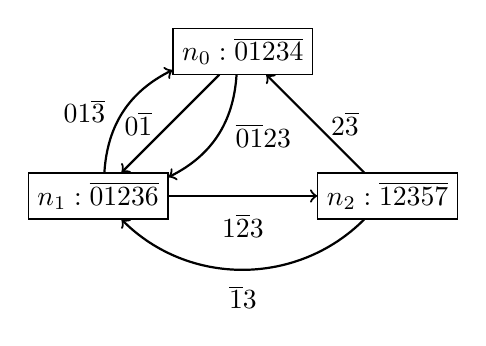
\begin{tikzpicture}[node distance = 26mm]
  \node[draw] (n0) {$n_0:\overline{01234}$};
  \node[draw,below left of=n0] (n1) {$n_1:\overline{01236}$};
  \node[draw,below right of=n0] (n2) {$n_2:\overline{12357}$};

  \draw[->,thick] (n0) -- node[left=1mm]  {$0\overline{1}$} (n1);
  \draw [->,thick] (n0) to [bend right=-30] node[right=1mm]  {$\overline{01}23$} (n1);
  \draw [->,thick] (n1) to [bend right=-30] node[left=1mm]  {$01\overline{3}$} (n0);

  \draw [->,thick] (n1) -- node[below=1mm]  {$1\overline{2}3$} (n2);
  \draw [->,thick] (n2) to [bend right=-45] node[below=2pt]  {$\overline{1}3$} (n1);

  \draw [->,thick] (n2) -- node[right=2pt]  {$2\overline{3}$} (n0);
\end{tikzpicture}
\vfill
\end{minipage}

\end{figure}

\end{frame}

\begin{frame}{Example: Our favorite edge}
\begin{columns}
		\begin{column}{4cm}
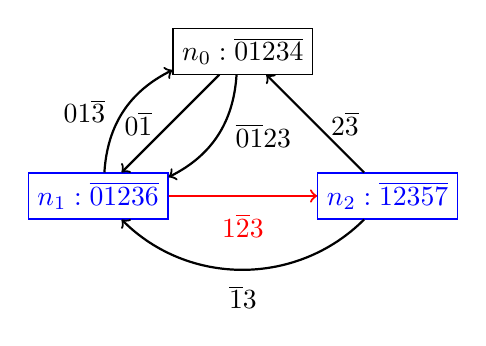
\begin{tikzpicture}[node distance = 26mm]
  \node[draw] (n0) {$n_0:\overline{01234}$};
 {\color{blue} \node[draw,below left of=n0] (n1) {$n_1:\overline{01236}$};}
 {\color{blue} \node[draw,below right of=n0] (n2) {$n_2:\overline{12357}$};}

  \draw[->,thick] (n0) -- node[left=1mm]  {$0\overline{1}$} (n1);
  \draw [->,thick] (n0) to [bend right=-30] node[right=1mm]  {$\overline{01}23$} (n1);
  \draw [->,thick] (n1) to [bend right=-30] node[left=1mm]  {$01\overline{3}$} (n0);

 {\color {red} \draw [->,thick] (n1) -- node[below=1mm]  {$1\overline{2}3$} (n2);}
  \draw [->,thick] (n2) to [bend right=-45] node[below=2pt]  {$\overline{1}3$} (n1);

  \draw [->,thick] (n2) -- node[right=2pt]  {$2\overline{3}$} (n0);
\end{tikzpicture}
\begin{center}
				\normalsize
				M1 $\to$ M6 \\
                M2 $\to$ M5 \\
                M3 $\to$ M4
				
			\end{center}
\end{column}

\begin{column}{5cm}
\begin{itemize}
\item Activity constraint. \newline
\pause 
$1{\color{lavenderindigo}\overline{2}}3$ : \textbf{M2} is active.
\pause
\item Fusion constraint. \newline
\pause
\textbf{M2, M5} are active. 
\pause
\item Pairing function. \newline
\pause 
\textbf{M2, M5} form a pair.
\pause
\item Steady state constraint. 
\end{itemize}
\end{column}
\end{columns}
\end{frame}


\begin{frame}{Example: Our favorite edge}
\begin{columns}
		\begin{column}{4cm}
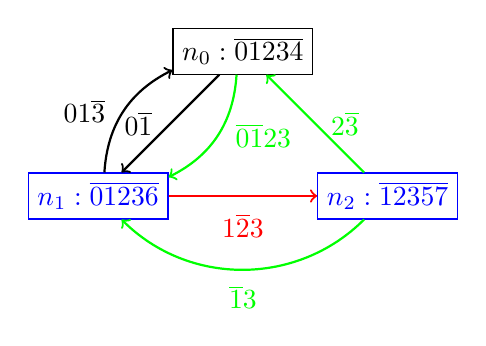
\begin{tikzpicture}[node distance = 26mm]
  \node[draw] (n0) {$n_0:\overline{01234}$};
 {\color{blue} \node[draw,below left of=n0] (n1) {$n_1:\overline{01236}$};}
 {\color{blue} \node[draw,below right of=n0] (n2) {$n_2:\overline{12357}$};}

  \draw[->,thick] (n0) -- node[left=1mm]  {$0\overline{1}$} (n1);
{\color {green}  \draw [->,thick] (n0) to [bend right=-30] node[right=1mm]  {$\overline{01}23$} (n1);}
  \draw [->,thick] (n1) to [bend right=-30] node[left=1mm]  {$01\overline{3}$} (n0);

 {\color {red} \draw [->,thick] (n1) -- node[below=1mm]  {$1\overline{2}3$} (n2);}
 {\color {green} \draw [->,thick] (n2) to [bend right=-45] node[below=2pt]  {$\overline{1}3$} (n1);}

 {\color {green} \draw [->,thick] (n2) -- node[right=2pt]  {$2\overline{3}$} (n0);}
\end{tikzpicture}
\begin{center}
				\normalsize
				M1 $\to$ M6 \\
                M2 $\to$ M5 \\
                M3 $\to$ M4
				
			\end{center}
\end{column}

\begin{column}{5cm}
\begin{itemize}
\item Steady state constraint. \newline
\pause
\textbf{M1}, \textbf{M3} come back direct edge. \newline
\pause
\textbf{M2} comes back using node $n_0$. \newline
\pause
\item Connectivity constraint. \newline 

\end{itemize}
\end{column}
\end{columns}
\end{frame}

\begin{frame}{Example: Our favorite edge}
\begin{columns}
		\begin{column}{4cm}
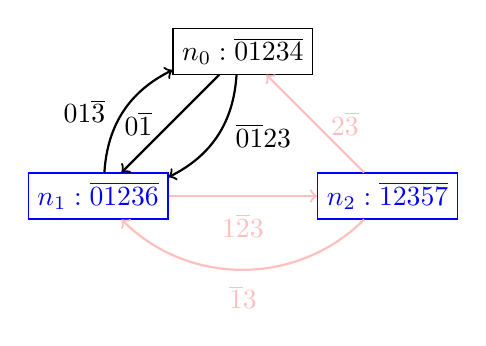
\begin{tikzpicture}[node distance = 26mm]
  \node[draw] (n0) {$n_0:\overline{01234}$};
 {\color{blue} \node[draw,below left of=n0] (n1) {$n_1:\overline{01236}$};}
 {\color{blue} \node[draw,below right of=n0] (n2) {$n_2:\overline{12357}$};}

  \draw[->,thick] (n0) -- node[left=1mm]  {$0\overline{1}$} (n1);
 \draw [->,thick] (n0) to [bend right=-30] node[right=1mm]  {$\overline{01}23$} (n1);
  \draw [->,thick] (n1) to [bend right=-30] node[left=1mm]  {$01\overline{3}$} (n0);

 {\color {pink}  \draw [->,thick] (n1) -- node[below=1mm]  {$1\overline{2}3$} (n2);}
 {\color {pink}  \draw [->,thick] (n2) to [bend right=-45] node[below=2pt]  {$\overline{1}3$} (n1);}

 {\color {pink}   \draw [->,thick] (n2) -- node[right=2pt]  {$2\overline{3}$} (n0);}
\end{tikzpicture}
\begin{center}
				\normalsize
				M1 $\to$ M6 \\
                M2 $\to$ M5 \\
                M3 $\to$ M4
				
			\end{center}
\end{column}

\begin{column}{5cm}
\begin{itemize}
\item Steady state constraint. \newline
M1, M3 come back direct edge. \newline
M2 comes back using node $n_0$. \newline
\item Connectivity constraint. \newline 
\pause 
Drop edge $d_{2,1}, d_{1,2}, d_{2,0}$.
\end{itemize}
\end{column}
\end{columns}
\end{frame}



% For a given k, size $\phi$, and molecule number $\sigma$, we are searching for well-structured, stable, and well-fused VTS G = (N, M, E, L, P, f)
%  such that N = $\phi$, M = $\sigma$, and G is not k-connected.
%\end{frame}

\section{Encodings}
% \begin{frame}
% Encoding for steady state condition and connectivity.
% \end{frame}

    \begin{frame} {Steady state Encoding}
    \textbf{Constraints for steady state condition.} \newline
    
``\textit{Every outgoing molecule come back in a cycle}''  \newline
 \hspace{2cm} \textbf{$\forall$ leaving m $\in$ M $\exists$ cycle [..]} \newline
\pause

Use {\color{blue} {reachability}} to encode the stability condition in VTSs.
  \begin{align}
 \bigwedge\limits_{i,j,m,p} r_{i,j,m,p} \implies (\, e_{i,j,m} \lor \bigvee_{i\neq i^{\prime}} ( \, e_{i,i^{\prime},m} \land r_{i^{\prime},j,m,p-1} ) )
  \tag{R}\label{eq:reach1}
\end{align}

$e_{i,j,m}$: an edge between node i and j contains molecule m.

$r_{i,j,m,p}$: a m-path from node i to j of length $\leq$ p.
\end{frame}
 
 \begin{frame}

Encode stability using the reachability variables.
% and say if there is an $m$-edge between $i$ and $j$, there is
% $m$-reachable path from $j$ to $i$.

\begin{align}
\bigwedge\limits_{i,j,m} ( e_{i,j,m} \implies r_{j,i,m,\mu})
% \bigwedge\limits_{i,j,m} (\bigvee_{q} e_{i,j,q,m}) \implies r_{j,i,m,\nu}
  \tag{2}\label{eq:reach2}
\end{align}
Number of molecules: $\mu$
    \end{frame}

 \begin{frame}[label=math]{$k$-connectivity constraints}
    The following constraints encode that only
existing edges can be dropped and exactly $k-1$ edges are dropped.
     \begin{equation}
\begin{alignedat}{2}
\ \bigwedge\limits_{i,j} d_{i,j} \implies e_{i,j}\\
  \sum_{i,j} d_{i,j} = k-1
\end{alignedat}
\end{equation}
but, in my opinion.
\begin{equation}
\begin{alignedat}{2}
\bigwedge\limits_{i,j}  [(e_{i,j} \land  \neg d_{i,j}) \lor  (\bigvee_{i' \neq i}  r^{\prime}_{i',j} \land  (e_{i,i'} \land \neg d_{i,i'}) ] \implies r^{\prime}_{i,j}  
\end{alignedat}
\end{equation}

 \begin{equation}
\begin{alignedat}{2}
 \bigvee\limits_{i,j} \neg (r^{\prime}_{i,j} \lor r^{\prime}_{j,i})
\end{alignedat}
\end{equation}
\end{frame}

% \begin{frame}[fragile]
% \frametitle{Fonts and Styles}
% \begin{figure}
% \includegraphics[height=3.5cm]{4.png}
% \end{figure}
%\end{frame}
\section{Results}
\begin{frame}{Results}
\begin{table}[t]
\centering
% \def\arraystretch{1.6}
  \begin{tabular}{|c|c|c|c|}
    \hline
    {\multirow{2}{*}{\textbf{Variant}}}  & 
    \multicolumn{2}{c|}{\textbf{Constraints}} & 
    {\multirow{2}{*}{\textbf{Graph connectivity}}}
    % \multicolumn{2}{c|}{\textbf{Graph connectivity}}
    \\
   \cline{2-3}
   &  \textbf{Rest} & \textbf{Activity} &  % & \textbf{Sampling: Guarantee}
\\ \hline
    
A. & \multirow{5}{*}{F + P + SS + C} 
     & N + N & No graph     \\\cline{3-4}
B. & & $\booleans$ + N & No graph     \\\cline{3-4}
C. & & N + $\booleans$ & {\color{blue} 3-connected}  \\\cline{3-4}
D. & & $\booleans$ + $\booleans$ & 2-connected  \\\cline{3-4}
E. & & N + P & No graph  \\\cline{3-4}
F. & & $\booleans$ + P &  {\color{blue} 4-connected}  \\\hline

% C_es :Self edges are allowed
% C_ed : Every edge is distinct 
  \end{tabular}
%\caption{{\bf Activity regulation of molecules vs. graph connectivity.}}
\label{tab:grph}
\end{table}
N: No regulation. Every present molecule is active. \newline
$\booleans$: Use boolean function for regulation. \newline
P: Use pairing matrix for regulation.
\end{frame}


% \begin{frame}[fragile]
% \textbf{Regulation on node: None, edge: Boolean function.}

% \begin{figure}
% \centering
% \begin{minipage}[b][5cm][s]{.45\textwidth}
% \centering
% \vfill
% %\begin{tikzpicture}[]
% \[
%  \begin{tikzpicture}[]
%  \matrix[mymatrix] (m)  {
%  \times & \times & \times &\times&\times&\times & \times & \times\\
% \times & \times & \times&\times&\times&\times& 1 &\times \\
% \times & \times & \times&\times&\times&1&\times &\times\\
% \times & \times & \times&\times & 1 & \times &\times & \times\\
%  \times & \times & \times & \times & \times & \times & \times & \times\\
%  \times & \times & \times &\times & \times & \times & \times & \times\\
%  \times & \times & \times & \times & \times & \times & \times & \times\\
%  \times & \times & \times & \times & \times & \times&\times & \times\\};
%   \mymatrixbraceright{1}{4}{$Q$}
%     \mymatrixbraceright{5}{8}{$R$}
%     \mymatrixbracetop{1}{4}{$Q$}
%     \mymatrixbracetop{5}{8}{$R$}
% \end{tikzpicture}
% \]
% \vfill
% %\caption{Pairing Matrix.}\label{fig:simple2}
% \vspace{\baselineskip}
% \end{minipage}\qquad
% \begin{minipage}[b][5cm][s]{.45\textwidth}
% \centering
% \vfill
% \begin{tikzpicture}[node distance = 26mm]
%   \node[draw] (n0) {$n_0:\overline{01234}$};
%   \node[draw,below left of=n0] (n1) {$n_1:\overline{01236}$};
%   \node[draw,below right of=n0] (n2) {$n_2:\overline{12357}$};

%   \draw[->,thick] (n0) -- node[left=1mm]  {$0\overline{1}$} (n1);
%   \draw [->,thick] (n0) to [bend right=-30] node[right=1mm]  {$\overline{01}23$} (n1);
%   \draw [->,thick] (n1) to [bend right=-30] node[left=1mm]  {$01\overline{3}$} (n0);

%   \draw [->,thick] (n1) -- node[below=1mm]  {$1\overline{2}3$} (n2);
%   \draw [->,thick] (n2) to [bend right=-45] node[below=2pt]  {$\overline{1}3$} (n1);

%   \draw [->,thick] (n2) -- node[right=2pt]  {$2\overline{3}$} (n0);
% \end{tikzpicture}
% \vfill
% \end{minipage}

% \end{figure}

% \end{frame}



\begin{frame}{Run-times for searching for models (in secs)}

\begin{table}[t]
  \centering
\adjustbox{max height=\dimexpr\textheight-5.5cm\relax,
           max width=\textwidth}{
\begin{tabular}[t]{|c|c|c|c|c|c|c|c|c|}\hline
  
    {\multirow{2}{*} {\textbf{Size}}}  & \multicolumn{2}{c|}{\textbf{Variant A}} & \multicolumn{2}{c|}{\textbf{Variant C}} & \multicolumn{2}{c|}{\textbf{Variant D}}  &  \multicolumn{2}{c|}{\textbf{Variant F}} \\\cline{2-9}
  
   {} & \multicolumn{2}{c|}{\textbf{2-connected} } & \multicolumn{2}{c|}{\textbf{3-connected} } & \multicolumn{2}{c|}{\textbf{2-connected}}  &  \multicolumn{2}{c|}{\textbf{4-connected}}
   %{} & \multicolumn{2}{c|}{2-connected} & \multicolumn{2}{c|}{3-connected} & \multicolumn{2}{c|}{2-connected}  &  \multicolumn{2}{c|}{4-connected}
   \\\cline{2-9}
    {} & {\textbf{MAA}} & {\textbf{Old-e}} & {\textbf{MAA}} & {\textbf{Old-e}} & {\textbf{MAA}} & {\textbf{Old-e}} & {\textbf{MAA}} & {\textbf{Old-e}} \\\hline
    2 & !0.085 & !2.43 & 0.15 & 2.12 & !0.13 & !1.89 & 0.35 & 5.12 \\\hline
    3 & !0.54 & !8.04 & 0.95  & 7.65 & 0.62 & 7.66  & 1.36 & 23.94\\\hline
    4 & !2.57 & !297.93 & 2.33 & 22.74 & 2.85 & 48.35  & 4.81 & 123.34\\\hline
    5 & !7.7 & !3053.8 & 7.60 & 500.03 & 10.27 & 890.84 & 33.36  & 2482.71 \\\hline
    6 & !22.98 & M/O & 19.52 & M/O & 30.81 & M/O  & 147.52 & M/O\\\hline
    7 & !57.07 & M/O & 81.89 & M/O & 82.94 & M/O & 522.26  & M/O \\\hline
    8 & !164.14 & M/O & 630.85 & M/O & 303.19 & M/O & 2142.76 & M/O\\\hline
    9 & !307.67 & M/O & 2203.45 & M/O & 971.01 & M/O & 4243.34 & M/O\\\hline
    10 & !558.34 & M/O & 7681.93 & M/O & 2274.30 & M/O & 7786.82 & M/O\\\hline
  \end{tabular}}
 % \caption{Run-times for searching for models (in secs).}
  \label{tab:qf-grabh}
\end{table}
\end{frame}

% \begin{frame}[fragile]{Bibliography}
% \bibliographystyle{plain}
% \bibliography{biblio.bib}
% \end{frame}

\section{Conclusion}
	
    \begin{frame}{Conclusion}
% 		\begin{columns}
% 			\begin{column}{4cm}
% 				\begin{figure}
%    					\includegraphics[height=4cm,width=5.5cm]{1.jpg}
% 				\end{figure}
% 			\end{column}
% 			\begin{column}{5cm}
            \begin{enumerate}
            \item Novel {\color{red}{encodings}} of reachability and 3-4 connectivity.
             \item Direct encoding into the SMT solver.
            \item A user friendly and scalable tool based on well known SMT solver Z3.
            \end{enumerate}
% 				\begin{flushright}
% 					\textit{}
% 					\vskip 0.5cm
% 				-- Mukund thattai
% 				\end{flushright}
% 			\end{column}
% 		\end{columns}
	\end{frame}

% \begin{frame}
% Contributions.
% 	\begin{figure}
%    		\includegraphics[height=4cm,width=4.5cm]{1.jpg}
% 	\includegraphics[height=4cm]{22.jpg}
%     \end{figure}
% \end{frame}

\end{document}
